\documentclass[oneside]{book}
\usepackage{ctex}
\usepackage[utf8]{inputenc}
\usepackage{amsmath}
%\usepackage{amsthm}
\usepackage{ntheorem}
\usepackage{booktabs}
\usepackage{caption}
\usepackage{listings}
\usepackage[dvipsnames]{xcolor}
\usepackage{xeCJK}
\usepackage{bm}
\usepackage{fancyhdr}
\usepackage{graphicx}
\usepackage{amssymb}
\usepackage{mathrsfs}
\usepackage{titlesec, blindtext, color}
\usepackage{arydshln}
\usepackage{hyperref} 
\usepackage[OT1]{fontenc}
\usepackage{geometry}
\usepackage{comment}
\usepackage{extarrows}
\usepackage{inconsolata}
\usepackage{enumitem}
\usepackage{ulem}

\geometry{
	a4paper,
	total={5in, 9in}
	}

\hypersetup{hidelinks,
	colorlinks=true,
	allcolors=black,
	pdfstartview=Fit,
	breaklinks=true
}

\fancyhf{}
\fancyhead[L]{
	\begin{minipage}[c]{0.06\textwidth}
		\hyperlink{Index}{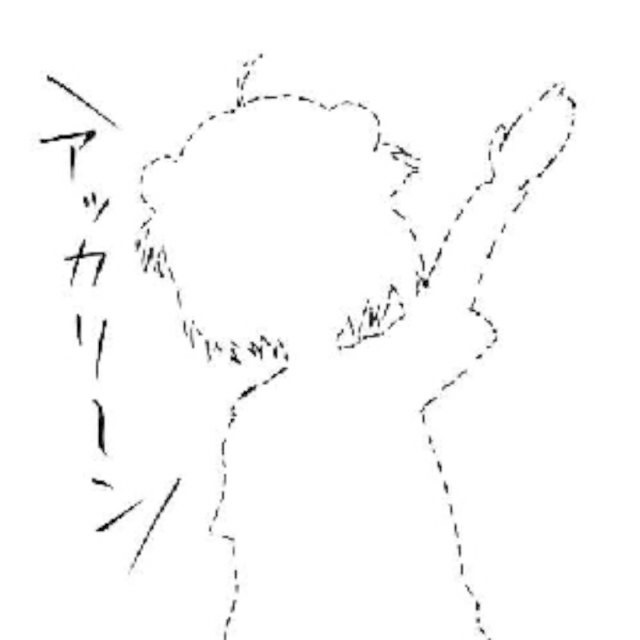
\includegraphics[height=7.5mm]{1.jpg}}
	\end{minipage}
	\begin{minipage}[c]{0.4\textwidth}
	英语大作文笔记
	\end{minipage}}
\fancyhead[R]{
    \begin{minipage}[r]{0.1\textwidth}
    \href{https://qifengggg.github.io/}{奇峰}
    \end{minipage}
}

%\cfoot{\thepage}
\cfoot{\hyperlink{Index}{\thepage}}
%\lfoot{\hyperlink{Index}{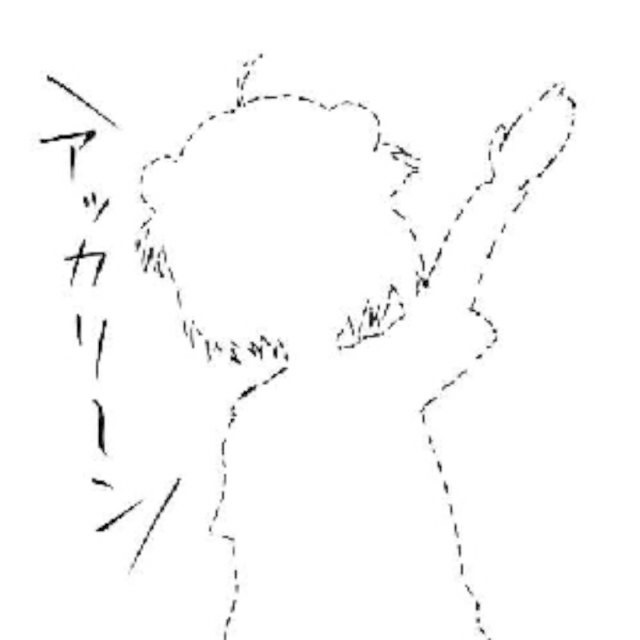
\includegraphics[height=7.5mm]{1.jpg}}}


\usepackage{titletoc}
\titlecontents{section}[4em]{\bfseries \zihao{5} \vspace{2pt}}
{\contentslabel{2em}}{\hspace*{-4em}}{~\titlerule*[0.6pc]{$.$}~\contentspage}


\begin{comment}
\titlecontents{subsection}[5em]{\zihao{5}}{\contentslabel{2em}}{\hspace*{-2em}}{~\titlerule*[0.6pc]{$.$}~\contentspage}
\titlecontents{subsubsection}[7em]{\zihao{5}}{\contentslabel{3em}}{\hspace*{-2em}}{~\titlerule*[0.6pc]{$.$}~\contentspage}
\titlecontents{paragraph}[11em]{\zihao{5}}{\contentslabel{4em}}{\hspace*{-2em}}{~\titlerule*[0.6pc]{$.$}~\contentspage}	
\end{comment}

\pagestyle{fancy}

\fancypagestyle{plain}{
  \fancyhead{}
  \renewcommand{\headrulewidth}{0pt}
}
%\renewcommand{\qedsymbol}{$\blacksquare$}

\renewcommand{\labelenumi}{\Roman{enumi}.}
\newcommand{\dis}{\displaystyle}
\newcommand{\Attention}[1]{\textcolor{red}{\bf{#1}}}
\newcommand{\sssubsection}[1]{\noindent\textbf{#1}}
\newcommand{\bs}{\blacksquare}
\newcommand{\ws}{\square}
\newcommand{\nextline}{\vspace{5pt}\newline}
\newcommand{\whichis}{\mathop=\limits^\Delta}
\newcommand{\atRight}[1]{\makebox[0.94\linewidth][r]{#1}}
\newcommand{\YS}{\makebox[0.94\linewidth][r]{Yours Sincerely,}}
\newcommand{\LM}{\makebox[0.94\linewidth][r]{Li Ming}}
\newcommand{\Chapter}[1]{\chapter{\hyperlink{Index}{#1}}}
\newcommand{\YSLM}{
	\YS
	
	\LM
}


\titleformat{\chapter}{\centering\Huge\bfseries\vspace{-2em}}{大作文}{0.5em}{}

\title{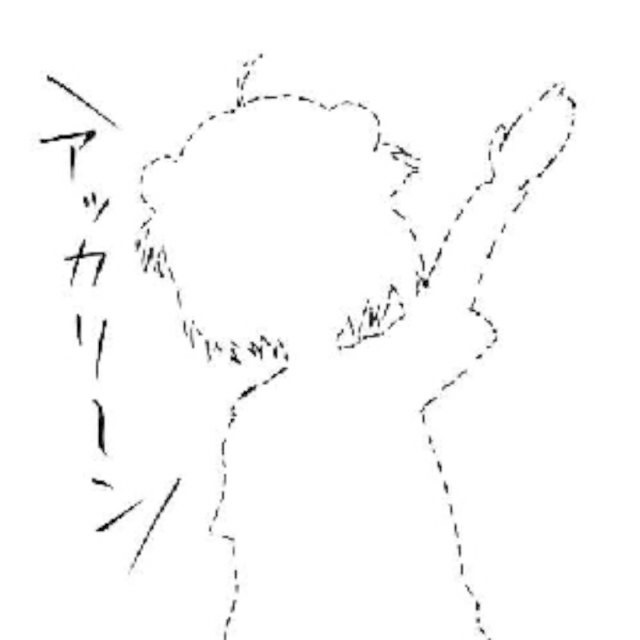
\includegraphics[scale=0.6]{1.jpg}\\ \textsf{英语大作文笔记}}
\author{\href{https://qifengggg.github.io/}{奇峰}}
\date{之前}

\begin{document}

\theoremseparator{}
\newtheorem{def1}{定义}[section]
\newtheorem{theo1}{定理}[section]
\newtheorem{func1}{方法}[section]
\newtheorem{infer1}{推论}[section]
\newenvironment{proof}[1][证明]{\noindent\newline\textbf{#1}\quad{}}{\hfill $\blacksquare$\par}
%\newenvironment{<环境名称>}[<参数个数>][<首参数默认值>]{<环境前定义>}
%							{<环境后定义>}



\newenvironment{Def}[1][\quad{}]{\begin{def1}\textbf{#1}}{\end{def1}}
\newenvironment{Theo}[1][\quad{}]{\begin{theo1}\textbf{#1}}{\end{theo1}}
\newenvironment{Func}[1][\quad{}]{\begin{func1}\textbf{#1}}{\end{func1}}
\newenvironment{Infer}[1][\quad{}]{\begin{infer1}\textbf{#1}}{\end{infer1}}
\newenvironment{Field}[1][\quad{}]{\noindent\newline\textbf{#1}}{}

\setlength{\parskip}{3pt}

\renewcommand{\labelitemii}{$ \circ $ }

\frontmatter
\maketitle
\hypertarget{Index}{}
\tableofcontents

\mainmatter

\chapter*{大作文的格式}

\section{行文逻辑}

\begin{itemize}
    \item \textbf{第一段}
    
    描述漫画内容。

    \begin{enumerate}[label = \Alph*.]
        \item 极简主义 - 抓住与漫画主题相关的细节;
        \item 时态 - 现在进行时、一般现在时;
        \item 汉语提示 - 不要直译
    \end{enumerate}
    \item \textbf{第二段}
    
    \textbf{论证某种品质的重要性;}

    阐述现象重要性;
    \item \textbf{第三段}
    
    提出建议,说明怎么做。
\end{itemize}

\newpage

\section{模板}

\subsection{单幅漫画}

A/An encouraging and thought-provoking story 
emerges from the image presented above: \textrm{(I)}
Apparently, the picture does mirror a common phenomenon in our contemporary society.

As a matter of fact, the picture
attempts to convey a crucial message:
\textrm{(I)} does count in \textrm{(I)} .
To put it more explicitly, it is undeniable that 
\textrm{(II)} (为什么需要XXX/XXX的重要性).
In such cases, \textrm{(III)} ought to \textrm{(III)}
(in order to \dots).
By contrast, should \textrm{(IV)} lack such awareness, \textrm{(IV)}
would be more likely to \textrm{(IV)} in the end.
A host of convincing examples can be found to illustrate my viewpoint.

On the whole, according to the analysis mentioned above, we could draw a reasonable 
conclusion that \textrm{(I)} are advised to cultivate/foster a sense of \textrm{(I)}
and put it into practice. Only in this manner can \textrm{(II)}.

%\newpage

\subsection{对比漫画}

The images pose a stark contrast:
in the first picture, \textrm{(I)}.
Conversely, in the second one, \textrm{(II)}.
Apparently, the drawing do reflect distinct attitudes and approaches 
adopted by different people in our contemporary society.

As a matter of fact, the pictures
attempt to convey a crucial message:
\textrm{(I)} does count in \textrm{(I)} .
To put it more explicitly, it is undeniable that 
\textrm{(II)} (为什么需要XXX/XXX的重要性).
In such cases, \textrm{(III)} ought to \textrm{(III)}
(in order to \dots).
By contrast, should \textrm{(IV)} lack such awareness, \textrm{(IV)}
would be more likely to \textrm{(IV)} in the end.
A host of convincing examples can be found to illustrate my viewpoint.

On the whole, according to the analysis mentioned above, we could draw a reasonable 
conclusion that \textrm{(I)} are advised to cultivate/foster a sense of \textrm{(I)}
and put it into practice. Only in this manner can \textrm{(II)}.
\chapter{行列式}

\sssubsection{定义与性质}

$$
    \begin{cases}
        \textrm{三大定义} 
        \begin{cases}
            &\textrm{几何定义};\\
            &\textrm{逆序定义};\\
            &\textrm{展开定义};\\
        \end{cases}
        \\
        \textrm{计算} 
        \begin{cases}
            &\textrm{数值形};\\
            &\textrm{含参形};\\
            &\Attention{\textbf{抽象形}};\\
        \end{cases}
        \\
        \textrm{证明} |A| = 0 
        \begin{cases}
            & |A| = -|A|;\\
            & r(A) < n;\\
            & \textrm{不可逆(常用于反证)};\\
            & AX = 0 \textrm{有非零解};\\
            & \exists \lambda_0 = 0;\\
        \end{cases}
        \\
    \end{cases}
$$ 

\section{求行列式的值}

\begin{itemize}
    \item 用性质消零(展开定义)
    \item 特殊行列式\begin{itemize}
        \item 三角形
        \item 范德蒙德行列式
        \item 分块
    \end{itemize}
    \item 特殊形状的行列式
\end{itemize}

\section{代数余子式}

代数余子式 $ A_{ij} = (-1)^{i+j}M_{ij}. $ 

注意,
\begin{itemize}
    \item 其为 $ (n-1) $ 阶子式;
    \item 其线性组合 $ \sum_i a_iA_ki $ 相当于将行列式第 $ k $ 行元素替换为 $ (a_i); $
    \item $ a_{i1}A_{j1} + a_{i2}A_{j2} + \cdots + a_{in}A_{jn} =
    \begin{cases}D,&i=j\\ 0,i\neq j\end{cases} $ 
    \item 伴随矩阵 $ A^* = \left(A_{ij}\right)^\top\whichis \Attention{|A|\cdot A^{-1}}$ 
\end{itemize}

对数值型矩阵 $ A, $ 求 $ A^* $ 时,可先求 $ |A| $ 并利用 $ (A\, \vdots\, E)\xrightarrow{\textrm{行变换}}
(E\, \vdots\, A^{-1}) $ 
求 $ A^{-1}, $ 再利用公式 $ A^* = |A|A^{-1} $ 求伴随矩阵。

\section{抽象矩阵行列式}

\sssubsection{性质}

\begin{enumerate}
    \item 对已知 $ A = (\alpha_i) $ 的矩阵,可以
    $ \begin{cases}
        \textrm{行列式列消}\\ \textrm{可逆时,}\begin{cases}
            \textrm{矩阵乘法}\\\textrm{相似}
        \end{cases}
    \end{cases} $ 
    \item $ |kA| = k^n|A|, $ 其中 $ k $ 可以是行列式;
    
    $ |A^\top|=A,|AB|=|A||B|=|B||A|=|BA|; $ 
    \item 设 $ A $ 可逆,则 $ A^* $ 可逆,且有

    $ |A^*| = |A|^{n-1};(A^*)^* = |A|^{n-2}A; $ 

    $ |(A^*)^*| = A^{(n-1)^2}; $ 
    \item $ |A| = \prod \lambda_i; tr(A) = \sum a_{ii} = \sum \lambda_i; $ 
    \item $ P^{-1}AP = B \Rightarrow |A| = |B|; $ 
    \item $ aA + bE $ 不可逆 $ \Leftrightarrow |aA + bE| = 0 \Rightarrow \exists \lambda_0 = \dfrac{-b}{a}; $ 
    \item $ AA^\top = A^\top A = E \Rightarrow |A| = \pm 1; $ 
    \item 对可逆矩阵 $ A, |A + \alpha\beta^T| = |A|(1+\beta^TA^{-1}\alpha); $ 
    
    对 $ B = \alpha\beta^T, |\lambda E + \alpha\beta^T| = \lambda^{n-1}(\lambda + \beta^\top\alpha); $ 
    \item 对 $ A_n, $ 若 $ A^2 = A,A\neq E, $ 则有 $ |A| = 0. $ \begin{itemize}
        \item 反证
        
        假设 $ A $ 可逆,则 $ A^2A^{-1} = AA^{-1} = E \Rightarrow A = E, $ 与题设矛盾,故
        $ A $ 不可逆,因此 $ |A| = 0. $ 
        \item 秩
        
        $ A^2 = A \Rightarrow A(A-E) = O \Rightarrow r(A) + r(A-E) \leq n;$
        
        $ A\neq E \Rightarrow r(A-E)>0 \Rightarrow r(A) < n \Rightarrow |A| = 0. $ 
        \item 方程组
        
        $ A^2 = A \Rightarrow A(A-E) = O; A \neq E \Rightarrow AX = O $ 存在非零解,
        因此 $ r(A)<n, $ 即 $ |A|=0. $ 
        \item 特征值
        
        $ A(A-E) = O = O(A-E),A\neq E, $ 因此 $ A $ 存在一特征值 $ \lambda_0 = 0, $ 
        此时 $ |A| = \prod \lambda = 0. $ 
    \end{itemize}
\end{enumerate}

其中,对于第八条,
\begin{enumerate}
    \item 有分块乘法
    \begin{equation*}
        \begin{aligned}
            &\begin{pmatrix}
                E&-\alpha\\0&1
            \end{pmatrix}
            \begin{pmatrix}
                A&\alpha\\-\beta^\top&1
            \end{pmatrix} = 
            \begin{pmatrix}
                A+\alpha\beta^\top & 0 \\ -\beta^T & 1
            \end{pmatrix}&(i)\\
            &\begin{pmatrix}
                E&0\\\beta^\top A^{-1} & 1
            \end{pmatrix}
            \begin{pmatrix}
                A&\alpha\\-\beta^\top&1
            \end{pmatrix} = 
            \begin{pmatrix}
                A & \alpha \\ 0 & 1+\beta^TA^{-1}\alpha
            \end{pmatrix}&(ii)\\
        \end{aligned}
    \end{equation*}
    显然 $ (i),(ii) $ 的两边也相等。此时对二者右边取得行列式,得到$$
    |A + \alpha\beta^T| = |A|(1+\beta^TA^{-1}\alpha)
    $$ 

    考虑一个例子 $ D = \begin{pmatrix}
        x+a_1 & a_2 & \cdots& a_n\\ 
        a_1 & x+a_2 & \cdots& a_n\\ 
        \vdots & \vdots & \ddots & \vdots \\ 
        a_1 & a_2 & \cdots & x+a_n
    \end{pmatrix} $ 
    
    显然其可以被拆分为 $ \begin{pmatrix}
        x&&&\\ &x&& \\ &&\ddots& \\ &&&x
    \end{pmatrix} $ 和 $ \begin{pmatrix}
        a_1 & a_2 & \cdots& a_n\\ 
        a_1 & a_2 & \cdots& a_n\\ 
        \vdots & \vdots & \ddots & \vdots \\ 
        a_1 & a_2 & \cdots & a_n
    \end{pmatrix} $ 
    
    此时可令前者为 $ A, $ 后者为 $ \alpha\beta^\top. $ 
    \item $ |\lambda E + \alpha\beta^\top| = |\lambda E - (-\alpha\beta^\top)|, $ 
    此时视 $ A = \lambda E, $ 
    
    套用前述方法有 $ |\lambda E + \alpha\beta^\top| = 
    |\lambda E|(1+\beta^T(\lambda E)^{-1}\alpha) = \lambda^{n}(1+\frac{\beta^\top\alpha}{\lambda})
    = \lambda^{n-1}(\lambda + \beta^\top\alpha). $ 
\end{enumerate}

注意,若有 $ AB=O,B = (\beta_i), $ 则考虑
\begin{itemize}
    \item $ r(A)+r(B)\leq n; $ 
    \item $ B $ 的列向量为 $ AX = O $ 的一组解;
    \item $ A\beta_i = O = O \beta_i, $ 此时 $ B $ 的列向量为 $ \lambda_A = 0 $ 的特征向量。
\end{itemize}

\sssubsection{计算抽象行列式}

计算抽象的行列式时,若其有法则,如 $ A^{-1},A^\top,A^*, $ 则利用其法则,
若其无法则,则利用 $ E = AA^{-1} $ 或 $ E = AA^\top. $

对求 $ |A+B| $ 的情况,由于无法则,考虑添加 $ E, $ 此时“一前一后,前者前,后者后。”对于

$$
    |A + B| = |E_1A + BE_2|,\ \ E_1,E_2 \textrm{都是单位矩阵}
$$ 

有\begin{itemize}
    \item $ E_1 $ 在 $ A $ 前,$ E_2 $ 在 $ B $ 后,此谓一前一后;
    \item $ E_1 $ 拆时,考虑同在前面的 $ B, $ 即 $ B^{-1}B $ 或 $ BB^{-1}, $ 此谓前者前;
    \item $ E_2 $ 拆时,考虑同在后面的 $ A, $ 即 $ A^{-1}A $ 或 $ AA^{-1}, $ 此谓后者后;
\end{itemize}

\sssubsection{由行列式值求参数}

需要加减·消元·出公因式。如
$$
    \begin{pmatrix}
        \lambda - 3 & 1 & -1 \\ 
        1 &\lambda -5 & 1 \\ 
        -1 & 1 & \lambda - 3
    \end{pmatrix}
    \xlongrightarrow{\textrm{第三列}-1\textrm{倍加到第一列}}
    \begin{pmatrix}
        \lambda - 2 & 0 & 2 - \lambda \\ 
        1 &\lambda -5 & 1 \\ 
        -1 & 1 & \lambda - 3
    \end{pmatrix}
$$ 

此时可以从第一列提出系数 $ \lambda - 2. $ 

\section{求行列式方程的根}

考察的方式可能为
\begin{itemize}
    \item 讨论根的个数 (行列式和最高次方)
    \item 根与系数的关系
    
    对 $ f(x) = D = \sum_{i = 0}^n a_i x^{n-i} $ 及其根 $ x_i $ 
    有 $ \begin{cases}
        \sum x_i = -\dfrac{a_1}{a_0} \\ 
        \prod (-x_i) = \dfrac{a_n}{a_0}
    \end{cases} $ 
\end{itemize}

\sssubsection{矩阵加边}

对行列式 $ D_n, $ 显然$$
    |D| = \left|
    \begin{array}{c:ccc}
        1&*&\cdots&*\\ \hdashline
        0& & & \\
        \vdots& &D& \\
        0& & & \\
    \end{array}
    \right|
$$ 

其中,为 $ * $ 的部分可以为任意值,因此可以按题面设置易于计算的值。另外,加入的一行
具体在哪一行都可以。

也可以通过加边构造行列式,使得其虽然不等于原式,但能通过性质辅助计算。如证明

$$
    D = \begin{vmatrix}
        1&1&1 &1 \\
        a_1^1&a_2^1 &a_3^1 &a_4^1 \\
        a_1^2&a_2^2 &a_3^2 &a_4^2 \\
        a_1^4&a_2^4 &a_3^4 &a_4^4 \\
    \end{vmatrix} = \sum a_i \prod (a_i - a_j)
$$ 

可以将其变为$$
    f(x) = \begin{vmatrix}
        x^0&1&1&1 &1 \\
        x^1&a_1^1&a_2^1 &a_3^1 &a_4^1 \\
        x^2&a_1^2&a_2^2 &a_3^2 &a_4^2 \\
        x^3&a_1^3&a_2^3 &a_3^3 &a_4^3 \\
        x^4&a_1^4&a_2^4 &a_3^4 &a_4^4 \\
    \end{vmatrix} \begin{matrix}
        \\ \\ \\ \leftarrow \textrm{增补行} \\ \\
    \end{matrix}
$$ 

并按照第一列展开,此时 $ x^3 $ 的系数$ A_3 $ 正好为 $ -|D|, $ 而
$ x^4 $ 的系数$ A_4 $ 为范德蒙德行列式,值为 $ \prod (x_i-x_j), $ 
由前述结论,$ \sum a_i = -\dfrac{A_3}{A_4}, $ 整理即得到结论。


\end{document}
